\documentclass[border=8pt]{standalone}
\usepackage{tikz}
\usetikzlibrary{arrows.meta,positioning,calc}
\begin{document}
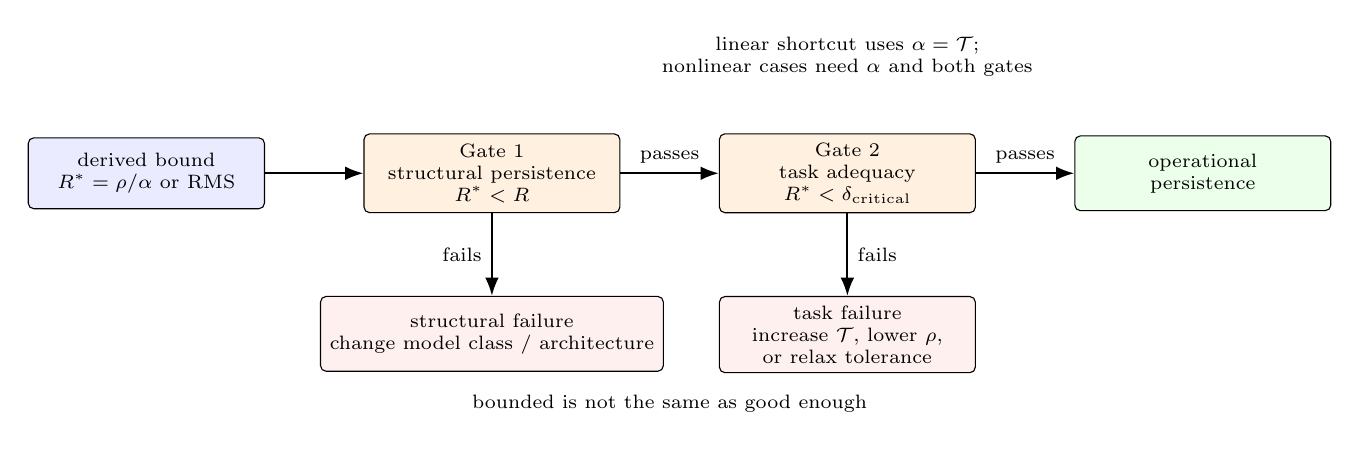
\begin{tikzpicture}[
  box/.style={draw, rounded corners=2pt, align=center, minimum width=3.0cm, minimum height=0.9cm, font=\scriptsize},
  gate/.style={draw, rounded corners=2pt, align=center, minimum width=3.25cm, minimum height=1.0cm, font=\scriptsize, fill=orange!12},
  fail/.style={draw, rounded corners=2pt, align=center, minimum width=3.25cm, minimum height=0.95cm, font=\scriptsize, fill=red!6},
  ok/.style={draw, rounded corners=2pt, align=center, minimum width=3.25cm, minimum height=0.95cm, font=\scriptsize, fill=green!8},
  arr/.style={-Latex, thick},
  note/.style={align=center, font=\scriptsize}
]

\node[box, fill=blue!8] (bound) {derived bound\\$R^\ast=\rho/\alpha$ or RMS};
\node[gate, right=1.25cm of bound] (struct) {Gate 1\\structural persistence\\$R^\ast<R$};
\node[gate, right=1.25cm of struct] (task) {Gate 2\\task adequacy\\$R^\ast<\delta_{\rm critical}$};
\node[ok, right=1.25cm of task] (op) {operational\\persistence};

\draw[arr] (bound) -- (struct);
\draw[arr] (struct) -- node[above, font=\scriptsize] {passes} (task);
\draw[arr] (task) -- node[above, font=\scriptsize] {passes} (op);

\node[fail, below=1.05cm of struct] (sfail) {structural failure\\change model class / architecture};
\node[fail, below=1.05cm of task] (tfail) {task failure\\increase $\mathcal T$, lower $\rho$,\\or relax tolerance};
\draw[arr] (struct) -- node[left, font=\scriptsize] {fails} (sfail);
\draw[arr] (task) -- node[right, font=\scriptsize] {fails} (tfail);

\node[note, below=0.65cm of $(sfail)!0.5!(tfail)$] {bounded is not the same as good enough};
\node[note, above=0.6cm of task] {linear shortcut uses $\alpha=\mathcal T$;\\nonlinear cases need $\alpha$ and both gates};

\end{tikzpicture}
\end{document}
